\chapter{Polarization of single top quarks in \textsl{t}~channel at 8~TeV}

\intro{A first measurement of the top quark spin asymmetry in t~channel, related to the top quark polarization, is presented in this chapter. Proton-proton collision data at $\mathit{\sqrt{s}=8}$~TeV have been analyzed corresponding to about $\mathit{20~fb^{-1}}$. Events with an isolated muon are selected together with two or three jets for the final measurement while events containing an isolated electron and jets have been studied as well. The normalized differential cross section is measured as a function of the polarization angle. From its shape, a spin asymmetry of $\mathit{0.26\pm0.03~(stat)\pm0.10~(syst)}$ is obtained. This is found to be compatible within $\mathit{2.0}$ standard deviations with the expected \gls{sm} asymmetry of $\mathit{0.44}$. The result has been published in Ref.~\cite{Khachatryan:2015dzz}. In a further step, the derivation of limits on anomalous couplings is illustrated by combining this measurement with related ones.}


An overview of the strategy to measure the top quark spin asymmetry and derive limits on anomalous couplings is given in the following. After selecting events with an isolated muon or electron and two or three jets, two \glspl{bdt} are employed. The first one, \bdtqcd, is trained to reject events with fake leptons stemming from multijet production. The amount of multijet contamination after the event selection is estimated through a two-component \gls{ml} fit to the \bdtqcd discriminant. The multijet background is modeled by a template obtained from data in a sideband region for which the lepton isolation is inverted. The second \gls{bdt}, \bdttch, is optimized to separate signal from \wjets and \ttbar events. The amount of signal and background fractions is estimate through a second \gls{ml} fit to its discriminant. A signal-enriched phase space is obtained by applying an optimized selection on each of the \glspl{bdt} discriminants resulting in a \gls{sb} ratio of about 90\%. The shape of the polarization angle, $\cos\theta^\star_{\mu}$, in data is unfolded to parton level after subtracting the remaining background contributions. This is repeated for each considered source of systematic uncertainty to estimate their impact on the measurement. The final measurement is performed in the muon channel only since in the electron channel, shortcomings in the modeling of the data-driven multijet template and an overall larger impact of systematic uncertainties are observed rendering its standalone result much less significant. The main focus is therefore set on the muon channel in the description of this analysis. From the differential cross section the asymmetry is obtained by a linear fit while accounting for the induced bin-by-bin correlations from the unfolding. The \TOPFIT program is utilized in a further step to derive limits on anomalous Wtb couplings by combining the measured asymmetry with an inclusive cross section measurement in $t$~channel and a measurement of the W~boson helicity fractions in \ttbar production.



%##############################################
\section{Event selection and simulated samples}
%##############################################
\label{sec:polarization-selection}

Proton-proton collision data at $\sqrt{s}=8~\TeV$ are analyzed corresponding to $19.7~\invfb$ recorded with the \gls{cms} experiment in 2012. Events are triggered on the presence of a single muon or electron candidate. The employed single muon trigger requires isolated muon candidates with $\pt>24~\GeV$ which fall within the pseudorapidity range of $|\eta|<2.1$. The single electron trigger fires when an electron candidate with $\pt>27~\GeV$ within $|\eta|<2.5$ is detected which has to fulfill some additional quality criteria corresponding to an efficiency of 80\% for prompt electrons. Motivated by the decay mode of the W~boson under the signal hypothesis, the events are categorized into ``channels'' depending if they have been triggered with the muon or electron trigger. For analysis, events in the muon channel have to contain one muon candidate with $\pt>26~\GeV$ within $|\eta|<2.1$ that passes the tight identification requirements. In the electron channel, events considered for analysis have to contain one electron candidate with $\pt>30~\GeV$ within $|\eta|<2.5$ that fulfills the tight \gls{mva}-based  identification. To suppress fake leptons from multijet production, the muon candidate has to have a relative \gls{deltabeta}-based isolation of $\muiso<12\%$ while the electron candidate has to have a relative \gls{effarea}-based isolation of $\eiso<10\%$. Events containing additional muons~($\pt>10~\GeV$, $|\eta|<2.5$) or electrons~($\pt>20~\GeV$, $|\eta|<2.5$) which pass corresponding loose identification criteria are rejected to suppress contributions from \zjets and dileptonic \ttbar production. 

Jets are clustered from \gls{pf} candidates with the anti-\kt algorithm using a distance parameter of $R=0.5$ while applying the \gls{chs} technique to remove the contamination of pileup tracks. \gls{pf} candidates belonging to preselected loosely isolated muons are not clustered into the jets to prevent double counting. In addition, jets which are within $\Delta R<0.3$ to the previous selected tight lepton are ignored in the analysis. The reconstructed jet energy in data and simulation and the energy resolution in simulation are calibrated through dedicated \gls{jec} and \gls{jer} scale factors. Events containing two or three jets with $\pt>40~\GeV$ that are detected within $|\eta|<4.5$ and pass loss identification criteria are considered for analysis. Tagging of jets which likely originated from the hadronization of a b~quark is performed with the \gls{csv} algorithm. Such jets are restricted to $|\eta|<2.4$ since the b-tagging algorithm operates only within the acceptance of the inner tracking system. An efficiency of about 50\% for tagging true b~jets with a mistagging rate of 0.1\% for other jets is found in simulation using the tight working point of the algorithm. The b-tagging efficiency is reweighted in simulation through scale factors to match the one measured in data. More details about the employed analysis objects, identification, and corrections have been described in Ch.~\ref{ch:reconstruction}.

Events are categorized as shown in Fig.~\ref{fig:polarization-categorization}. The different regions are labeled as ``$N\,\mathrm{j}~M\,\mathrm{t}$'' where $N$ denotes the number of selected jets and $M$ the subset of jets which are also b-tagged. Control regions dominated by either \wjets~(2j0t) or \ttbar~(3j1t, 3j2t) production are defined besides the signal region~(2j1t). The analysis was developed by validating the background modeling and optimizing the strategy by comparing to data in the control regions only. During this process, data in the signal region has not been used. This procedure is commonly referred to as ``blinding''. After the strategy is fixed the final measurement was conducted by unblinding the signal region while refraining from any further optimizations. The blinding procedure prevents a result-driven tuning of the analysis strategy which could bias the measurement.

\myfigure{\label{fig:polarization-categorization}Categorization of events depending on number of selected jets, number of b-tags, and the signal \gls{bdt} discriminant. The shaded regions are utilized in a template-based \gls{ml} fit as described in Sec.~\ref{sec:polarization-fit} for estimating the signal and background yields.}{
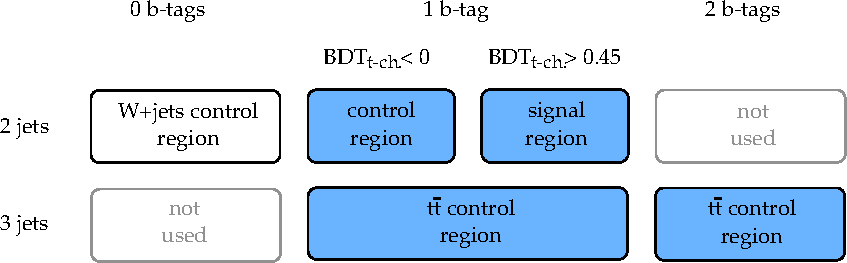
\includegraphics[scale=0.75]{figures/polarization/regions.pdf}
}

Various samples of simulated events for signal and background processes are generated. The default signal sample is generated in 5~\gls{fs} using the \POWHEG\,v1 generator interfaced with \PYTHIA\,6 for parton showering and \TAUOLA for tau decays. For comparisons, two additional, alternative signal samples are generated. One utilizes the \AMC generator interfaced with \PYTHIA\,8 in 4~\gls{fs} while the other employs the \COMPHEP generator interfaced with \PYTHIA\,6. A set of special samples with anomalous Wtb couplings is generated as well using the \COMPHEP generator for testing the analysis strategy. Samples containing single top quark events produced via tW and $s$~channel are generated with \POWHEG\,v1 interfaced with \PYTHIA\,6 and \TAUOLA. The major background processes, \wjets, \zjets, and \ttbar, are generated with the \MG generator interfaced with \PYTHIA\,6 and \TAUOLA as well. Samples with up to three~(\ttbar) or four~(\wjets,\zjets) additional partons at \gls{me} level are merged together using the \gls{mlm} merging procedure. For \wjets production, an alternative sample generated with \SHERPA~\cite{Hoeche:2012ft} is employed for validation purposes. In this thesis, \wjets events are categorized based on their jet flavor content. Events with at least one heavy-quark flavored jet from either c, or b~quarks are abbreviated as ``\glsmark{whf}'' while events with only light-quark flavored jets~(g,u,d,s) are labeled as ``\glsmark{wlf}'' instead. Diboson production~(WW,WZ,ZZ) is a minor background and simulated with \PYTHIA\,6. The cross sections used to normalize the samples are listed in Tab.~\ref{tab:polarization-theo-xsecs}. Throughout this chapter the individual signal and background templates are scaled to the result of a binned \gls{ml} fit to data~(Sec.~\ref{sec:polarization-fit}) and corrections to the simulated \wjets and \ttbar events~(Sec.~\ref{sec:polarization-modeling}) are applied unless explicitly stated otherwise.


\mytable{\label{tab:polarization-theo-xsecs}Theoretical cross sections used to normalize the simulated samples.}{
\begin{tabular}{|l  r c l |}
\hline
process & $\sigma/\pb$ &\hspace{0.1cm} & accuracy \\
\hline
$t$~channel & $87.1~\pb$ & & approx. \gls{nnlo}~\cite{Kidonakis:2012db} \\
$s$~channel & $5.55~\pb$ && approx. \gls{nnlo}~\cite{Kidonakis:2012db}  \\
tW~channel & $22.2~\pb$ && approx. \gls{nnlo}~\cite{Kidonakis:2012db} \\
\ttbar & $252.9~\pb$ && \gls{nnlo} (using Top++\,2.0~\cite{Czakon:2011xx}) \\
$\mathrm{W}\to\ell\nu\mathrm{\,\mbox{+}\,jets}$ & $37\,509~\pb$ && \gls{nnlo} (using FEWZ~\cite{Gavin:2010az}) \\
$\mathrm{Z}/\gamma^{*}\to\ell^{\rmplus}\ell^{\rmminus}$, $m_{\ell\ell}>50~\GeV$ & $3\,504~\pb$ && \gls{nnlo} (using FEWZ~\cite{Gavin:2010az}) \\
WW & $54.8~\pb$ && \gls{nlo} (using MCFM\,5.8~\cite{Campbell:2010ff})\\
WZ & $33.2~\pb$ && \gls{nlo} (using MCFM\,5.8~\cite{Campbell:2010ff})\\
ZZ & $8.1~\pb$ && \gls{nlo} (using MCFM\,5.8~\cite{Campbell:2010ff})\\
\hline
\end{tabular}
}

The fake lepton background stemming from multijet production is estimated from data in sideband regions for which the isolation of the lepton is inverted as $\muiso>20\%$ and $\eiso>15\%$, respectively. The distribution of data serves as a template of the shape of multijet production after subtracting the remaining contamination by other processes. Figure~\ref{fig:polarization-qcd-template} shows the distribution of the transverse W~boson mass in this sideband region and the resulting multijet template after it has been fitted to data in the 2j1t region of the muon channel. A purity of about 91\% (98\%) is found in muon (electron) channel respectively. The extracted template yields a good description of the unknown multijet shape in the signal region after scaling it to the result of a \gls{ml} fit as described below.

\myfigure{\label{fig:polarization-qcd-template}Distributions of the transverse W~boson mass in muon channel: (a)~antiisolated sideband region for extracting the multijet template; (b)~resulting distribution in the 2j1t region after scaling the extracted template to data through a \gls{ml} fit.}{
\subfloat[]{\adjincludegraphics[height=4.8cm,trim={0 0 {0.16\width} 0},clip]{figures/polarization/beforeBgCorr/2j1t/muon_2j1t_mtw_qcdnone_antiiso_nol.pdf}}
\subfloat[]{\adjincludegraphics[height=4.8cm,trim={0 0 {0.\width} 0},clip]{figures/polarization/afterBgCorr/2j1t/muon_2j1t_mtw_qcdnone.pdf}}
}

Distributions of the reconstructed top quark mass in muon and electron channel after the event selection are shown in Fig.~\ref{fig:polarization-topmass}. In control regions containing no or more than one b-tagged jet, the jet with the highest value of the \gls{csv} discriminant is associated to the top quark decay to calculate the top quark mass.  The presented distributions show that data is well described by the simulated events and the multijet templates in control and signal regions in electron and muon channel.

The distributions display a peak for the single top quark signal in 2j1t for a top quark mass range of about $150\range190~\GeV$ as expected. For \ttbar production, the selected b-tagged jet may not be always associated with the corresponding lepton from a top quark decay. Hence, its distributions shows a peak with a wider tail. Unfortunately, the event selection also leads to a similar shape for the \wjets background although it exhibits an even longer tail. In conclusion, it can be seen that a simple selection on the top quark mass is insufficient to select a signal-enriched phase space. Therefore, two \glspl{bdt} are trained for separating signal from background events as detailed in the next section.

\myfigure[p]{\label{fig:polarization-topmass} Distributions of the reconstructed top quark mass in (left column)~electron and (right column)~muon channel. Top row: 2j0t \wjets control region; middle row: 2j1t region; bottom row: 3j1t \ttbar control region. The top quark \pt reweighting~(Sec.~\ref{sec:polarization-modeling}) is exceptionally not applied here.}{
\subfloat[]{\adjincludegraphics[height=4.8cm,trim={0 0 {0.16\width} 0},clip]{figures/polarization/beforeBgCorr/2j0t/electron_2j0t_top_mass_qcdnone_nol.pdf}}
\subfloat[]{\adjincludegraphics[height=4.8cm,trim={0 0 {0.\width} 0},clip]{figures/polarization/beforeBgCorr/2j0t/muon_2j0t_top_mass_qcdnone.pdf}}\\
\subfloat[]{\adjincludegraphics[height=4.8cm,trim={0 0 {0.16\width} 0},clip]{figures/polarization/beforeBgCorr/2j1t/electron_2j1t_top_mass_qcdnone_nol.pdf}}
\subfloat[]{\adjincludegraphics[height=4.8cm,trim={0 0 {0.\width} 0},clip]{figures/polarization/beforeBgCorr/2j1t/muon_2j1t_top_mass_qcdnone.pdf}}\\
\subfloat[]{\adjincludegraphics[height=4.8cm,trim={0 0 {0.16\width} 0},clip]{figures/polarization/beforeBgCorr/3j2t/electron_3j2t_top_mass_qcdnone_nol.pdf}}
\subfloat[]{\adjincludegraphics[height=4.8cm,trim={0 0 {0.\width} 0},clip]{figures/polarization/beforeBgCorr/3j2t/muon_3j2t_top_mass_qcdnone.pdf}}
}



%##############################################
\section{Training of Boosted Decision Trees}
%##############################################
\label{sec:polarization-bdt-training}

Two \glspl{bdt} are trained to obtain a signal-enriched phase space. The first \gls{bdt}, labeled \bdtqcd, is trained to reject background events stemming from multijet production. Simulated $t$-channel single top quark events are set as signal class and data events from the sideband region where the multijet template is extracted are set as background class. The gradient boosting procedure is chosen for the training with a relatively low shrinkage of 10\%. The number of single decision trees is restricted to 50 while each tree is kept shallow with a maximum depth of two. The minimum node size is set to 250 events. These settings are not optimized to yield the best discrimination power but instead are motivated to protect well against overtraining. This a particular concern here since the usage of data events for training may not reflect the distribution of multijet events in the signal region to the extend as it would be with simulated events. Multiple \gls{bdt} candidates are trained to assess which set of discriminating input observables yields the best rejection of multijet events with the final discriminant. Correlated observables are excluded from the training by testing individually that the discrimination power does not diminish when removed. This resulted in the following list of five input observables:

\begin{itemize}
\item the reconstructed invariant mass of the top quark candidate;
\item the transverse mass of the W~boson candidate before solving for the unknown neutrino $p_{z}$ component since this modifies \pvmiss in case of complex solutions, \mtw;
\item the missing transverse energy, \met;
\item the transverse momentum of the untagged spectator jet~(\jprime);
\item the event isotropy which is defined as $(s_\mathrm{max}-s_\mathrm{min})/s_\mathrm{max}$ with $s=\sum_{i}^\scriptn{\ell,\,\mathrm{jets}}\big|\,\vec{n}\cdot\vec{p}_{i}\big|$ where the unit vector $\vec{n}=(\cos\phi,\sin\phi)$ is chosen in the transverse plane such that it either maximizes or minimizes $s$.
\end{itemize}

Distributions of \mtw, $\jprime~\pt$, and the event isotropy are presented in Fig.~\ref{fig:polarization-qcdinputs} while the other input observables are shown in Figs.~\ref{fig:polarization-qcd-template} and~\ref{fig:polarization-topmass} above. The distribution of the resulting \gls{bdt} discriminant is shown Fig.~\ref{fig:polarization-bdt-qcd}. A fair agreement is observed between data and simulation.

\myfigure{\label{fig:polarization-qcdinputs}Distributions of some input observables of the \bdtqcd and \bdttch discriminants as indicated in 2j1t muon channel: (a)~missing transverse energy; (b)~transverse momentum of untagged spectator jet; (c)~event isotropy; (d)~transverse momentum of b~tagged jet.}{
\subfloat[\bdtqcd and \bdttch]{\adjincludegraphics[height=4.8cm,trim={0 0 {0.16\width} 0},clip]{figures/polarization/afterBgCorr/2j1t/muon_2j1t_met_qcdnone_nol.pdf}}
\subfloat[\bdtqcd and \bdttch]{\adjincludegraphics[height=4.8cm,trim={0 0 {0.\width} 0},clip]{figures/polarization/afterBgCorr/2j1t/muon_2j1t_ljet_pt_qcdnone.pdf}}\\
\subfloat[only \bdtqcd]{\adjincludegraphics[height=4.8cm,trim={0 0 {0.16\width} 0},clip]{figures/polarization/afterBgCorr/2j1t/muon_2j1t_isotropy_qcdnone_nol.pdf}}
\subfloat[only \bdttch]{\adjincludegraphics[height=4.8cm,trim={0 0 {0.\width} 0},clip]{figures/polarization/afterBgCorr/2j1t/muon_2j1t_bjet_pt_qcdnone.pdf}}
}

In a preliminary version of this analysis~\cite{CMS-PAS-TOP-13-001}, events with $\mtw>50~\GeV$ ($\met>45~\GeV$) are selected in muon (electron) channel respectively to reject multijet events. Here, the working points of the \bdtqcd discriminant have been chosen such that similar signal selection efficiencies are obtained per channel. A comparison of the working point performances is presented in Tab.~\ref{tab:polarization-qcdeff}. The usage of the new \bdtqcd with respect to the preliminary analysis allows to reject about twice as much multijet events while retaining approximately the same amount of signal events.

\mytable{\label{tab:polarization-qcdeff}Selection efficiencies of multijet and signal events using \bdtqcd, \mtw, and \met working points where the latter two were used in a preliminary version of the analysis.}{
\begin{tabular}{|r | c c | c c |}
\hline
& \multicolumn{2}{c|}{Muon channel} & \multicolumn{2}{c|}{Electron channel}\\
Process    & $\mtw>50~\GeV$ & $\bdtqcd>-0.15$ & $\met>45~\GeV$ & $\bdtqcd>0.15$ \\
\hline
Multijet  & 15\% & 7.7\%  & 7.6\% & 4.4\% \\
Signal   & 70\% & 71\%   & 51\%  & 52\% \\
\hline
\end{tabular}
}

The second \gls{bdt}, \bdttch, is trained to separate signal events from \wjets and \ttbar production which are the major background processes after applying the multijet rejection selection. It is configured as follows. The gradient boosting method is employed with a shrinkage of 40\%. In total, 200~shallow single decision trees with a maximum depth of two are trained. The minimum node size is set to 100 events. To mitigate a potential lack in the training statistics of the backgrounds, additional simulated \wjets and \ttbar events from the 2j0t and 3j2t control regions are added to the training, respectively. In particular, this increases the statistics of W+light flavored jets which is relatively low in simulation in the 2j1t region but may in fact be larger in data due to mistagging. The following ten observables have been chosen as input:

\begin{itemize}
\item the reconstructed invariant mass of the top quark candidate;
\item the missing transverse energy, \met;
\item the transverse mass of the W~boson candidate before solving for the unknown neutrino $p_{z}$ component, \mtw;
\item the transverse momentum of the lepton;
\item the transverse momentum of the b-tagged jet;
\item the invariant mass of the b-tagged jet from the summed momenta of the clustered \gls{pf} candidates;
\item the absolute pseudorapidity of the untagged spectator jet~(\jprime);
\item the absolute pseudorapidity of the b-tagged jet;
\item the invariant mass of the top quark and spectator jet system, $\sqrt{\hat{s}}=\big|\vec{p}_{\mathrm{top}}+\vec{p}_{\jprime}\big|$\,;
\item the transverse momentum of the hadronic final-state system~(\glsmark{hfs}), $\big(\vec{p}_{\jprime}+\vec{p}_{\mathrm{b}}\big)_\mathrm{T}$\,.
\end{itemize}

These observables have been chosen because they exhibit a low correlation with the polarization angle. A bias may otherwise occur since the \gls{bdt} is trained with a sample of simulated signal events with a \gls{sm} coupling structure. In the worst case, the \gls{bdt} may select events in such a way that it artificially reproduces the shape of the expected polarization angle in data. Choosing uncorrelated observables makes the \gls{bdt} training blind to the actual distribution of the polarization angle instead. The distributions of some input observables are shown in Fig.~\ref{fig:polarization-tchinputs} after selecting events with $\bdtqcd>-0.15$ in 2j1t muon channel. The remaining ones are presented in Figs.~\ref{fig:polarization-qcd-template}, \ref{fig:polarization-topmass}, and~\ref{fig:polarization-qcdinputs} above. The resulting discriminant is shown in Fig.~\ref{fig:polarization-bdt-tch} in 2j1t muon channel. Overall, a good description of data with simulation is observed.

\myfigure{\label{fig:polarization-bdts}Distributions of the \glspl{bdt} discriminants in 2j1t muon channel: (a)~multijet \gls{bdt}; (b)~signal \gls{bdt} after rejecting multijet events.}{
\subfloat[\label{fig:polarization-bdt-qcd}]{\adjincludegraphics[height=4.8cm,trim={0 0 {0.16\width} 0},clip]{figures/polarization/afterBgCorr/2j1t/muon_2j1t_bdt_qcd_qcdnone_nol.pdf}}
\subfloat[\label{fig:polarization-bdt-tch}]{\adjincludegraphics[height=4.8cm]{figures/polarization/afterBgCorr/2j1t/muon_2j1t_bdt_tch_qcdbdt.pdf}}
}

\myfigure[p]{\label{fig:polarization-tchinputs}Distributions of some input observables to the \bdttch discriminant in 2j1t muon channel: (a)~transverse momentum of the muon; (b)~invariant mass of the b-tagged jet; (c,d)~absolute value of the untagged and b-tagged jet pseudorapidities; (e)~invariant mass of the top quark and spectator jet system; (f)~\pt of the hadronic final state system.}{
\subfloat[]{\adjincludegraphics[height=4.8cm,trim={0 0 {0.16\width} 0},clip]{figures/polarization/afterBgCorr/2j1t/muon_2j1t_lepton_pt_qcdbdt_nol.pdf}}
\subfloat[]{\adjincludegraphics[height=4.8cm,trim={0 0 {0.\width} 0},clip]{figures/polarization/afterBgCorr/2j1t/muon_2j1t_bjet_mass_qcdbdt.pdf}}\\
\subfloat[]{\adjincludegraphics[height=4.8cm,trim={0 0 {0.16\width} 0},clip]{figures/polarization/afterBgCorr/2j1t/muon_2j1t_ljet_abseta_qcdbdt_nol.pdf}}
\subfloat[]{\adjincludegraphics[height=4.8cm]{figures/polarization/afterBgCorr/2j1t/muon_2j1t_bjet_abseta_qcdbdt.pdf}}\\
\subfloat[]{\adjincludegraphics[height=4.8cm,trim={0 0 {0.16\width} 0},clip]{figures/polarization/afterBgCorr/2j1t/muon_2j1t_shat_mass_qcdbdt_nol.pdf}}
\subfloat[]{\adjincludegraphics[height=4.8cm,trim={0 0 {0.\width} 0},clip]{figures/polarization/afterBgCorr/2j1t/muon_2j1t_hfs_pt_qcdbdt.pdf}}
}


%##############################################
\section{Background modeling}
%##############################################
\label{sec:polarization-modeling}

The modeling of the \wjets and \ttbar backgrounds is studied in control regions before performing the measurement. In the 2j0t control region, two mismodeled observables are found which can be attributed to the \wjets background, after applying the \bdtqcd selection to reject the multijet background. 

The transverse momentum of the W~boson displays a softer spectrum in data compared to simulation as shown in Fig.~\ref{fig:polarization-wjets-reweighting-wpt}. This effect can be explained as an insufficient modeling of the hadronic recoil in such events. The recoil momentum is defined for \zjets and \wjets events as the net momentum which balances the momentum of the vector boson in the transverse plane. It is mostly the vectorial sum of hard jets but has also a soft contributions stemming from the underlying event, bremsstrahlung photons, and pileup. In this analysis, a simple reweighting of simulated events in bins of the W~boson \pt is applied to correct for this deviation. More sophisticated methods can be found in literature (e.g. Ref.~\cite{Abazov:2009tra}). The W~boson \pt scale factors derived in the 2j0t control region are also applied in the 2j1t signal region. In the statistical evaluation, the difference between applying and not applying this reweighting is considered as a systematic uncertainty.

\myfigure{\label{fig:polarization-wjets-pt}Distributions of the reconstructed W~boson \pt in 2j0t control region: (a)~before and (b)~after applying the \wjets corrections.}{
\subfloat[\label{fig:polarization-wjets-reweighting-wpt}]{\adjincludegraphics[height=4.8cm,trim={0 0 {0.16\width} 0},clip]{figures/polarization/beforeBgCorr/2j0t/muon_2j0t_wboson_pt_qcdbdt_nol.pdf}}
\subfloat[\label{fig:polarization-wjets-reweighting-wpt-rew}]{\adjincludegraphics[height=4.8cm,trim={0 0 {0.\width} 0},clip]{figures/polarization/afterBgCorr/2j0t/muon_2j0t_wboson_pt_qcdbdt.pdf}}
}

Another mismodeling of the \wjets background is observed for the polarization angle itself which is presented in Fig.~\ref{fig:polarization-wjets-reweighting-cosTheta}. This is a percuiliar mismodeling since $\cos\theta_\mu^\star$ does not reflect a physically meaningful observable for \wjets events. A similar deviation has been observed in measurements at 7~TeV as well~\cite{Komm-thesis}. The modeling is cross checked using an alternative \wjets sample simulated with the \SHERPA generator. This sample was however simulated with only massless quarks. Hence the ratio of light, charm, and bottom flavored jets is predicted wrongly. The flavor ratios are therefore reweighted to the ones predicted by the default \MG sample. The distributions before and after the reweighting are shown in Fig.~\ref{fig:polarization-sherpa-cosTheta}. A better modeling of $\cos\theta_{\mu}^\star$ but with a somewhat opposite trend compared to Fig.~\ref{fig:polarization-wjets-cosTheta} is obtained. For the measurement, the shape of $\cos\theta_{\mu}^\star$ is reweighted using \MG-to-\SHERPA scale factors per jet flavor derived in 2j0t control region which are applied in the signal region as well. The resulting distribution in 2j0t is shown in Fig.~\ref{fig:polarization-wjets-reweighting-cosTheta-rew} where a fair description of data is achieved. Two additional systematic uncertainties are considered in the measurement to account for the difference between the two $\cos\theta_\mu^\star$ shapes and the flavor composition of the \wjets sample.

In the measurements at 13~\TeV~(Ch.~\ref{ch:diff13}), the \wjets background is simulated at \gls{nlo} using the \MGAMC generator which yields an improved modeling of data in the 2j0t control region. In retrospect, the observed mismodeling here may therefore be judged as a consequence of the \gls{lo} accuracy of the \MG \wjets sample.

\myfigure{\label{fig:polarization-wjets-cosTheta}Distributions of the polarization angle in 2j0t control region: (a)~before and (b)~after applying the \wjets corrections.}{
\subfloat[\label{fig:polarization-wjets-reweighting-cosTheta}]{\adjincludegraphics[height=4.8cm,trim={0 0 {0.16\width} 0},clip]{figures/polarization/beforeBgCorr/2j0t/muon_2j0t_cosTheta_lj_qcdbdt_nol.pdf}}
\subfloat[\label{fig:polarization-wjets-reweighting-cosTheta-rew}]{\adjincludegraphics[height=4.8cm,trim={0 0 {0.\width} 0},clip]{figures/polarization/afterBgCorr/2j0t/muon_2j0t_cosTheta_lj_qcdbdt.pdf}}
}

\myfigure{\label{fig:polarization-sherpa-cosTheta}Distributions of the polarization angle in 2j0t control region using an alternative \wjets sample simulated with \SHERPA: (a)~before and (b)~after reweighting the jet flavor fractions to the predictions by \MG.}{
\subfloat[\label{fig:polarization-sherpa-reweighting-cosTheta}]{\adjincludegraphics[height=4.8cm,trim={0 0 {0.16\width} 0},clip]{figures/polarization/sherpa_nofl/muon_2j0t_cosTheta_lj_qcdbdt_nol.pdf}}
\subfloat[\label{fig:polarization-sherpa-reweighting-cosTheta-rew}]{\adjincludegraphics[height=4.8cm,trim={0 0 {0.\width} 0},clip]{figures/polarization/sherpa_fl/muon_2j0t_cosTheta_lj_qcdbdt.pdf}}
}

After applying the described \wjets corrections an improved modeling can also be observed for other observables. Figure~\ref{fig:polarization-wjets-reweighting-met} shows the distribution of \met before and after applying the corrections. 

\myfigure{\label{fig:polarization-wjets-reweighting-met}Distribution of \met in mon channel 2j0t control region for (a)~before and (b)~after applying the \wjets corrections.}{
\subfloat[]{\adjincludegraphics[height=4.8cm,trim={0 0 {0.16\width} 0},clip]{figures/polarization/beforeBgCorr/2j0t/muon_2j0t_met_qcdnone_nol.pdf}}
\subfloat[]{\adjincludegraphics[height=4.8cm,trim={0 0 {0.\width} 0},clip]{figures/polarization/afterBgCorr/2j0t/muon_2j0t_met_qcdnone.pdf}}
}


In the \ttbar control region, the reconstructed top quark \pt displays a softer spectrum in data than predicted by simulation as shown in Fig~\ref{fig:polarization-toppt}. Such a deviation is also observed in differential \ttbar cross section measurements~\cite{Chatrchyan:2012saa,Khachatryan:2015oqa}. To mitigate this an ad-hoc recipe for calculating a per event weight as

\begin{equation}
w=\sqrt{\mathrm{SF}\big(\pt(\mathrm{t})\big)\cdot\mathrm{SF}\big(\pt(\bar{\mathrm{t}})\big)}\,,
\end{equation} 

is applied for simulated \ttbar events where the weight depends on the transverse top quark and antiquark momenta at parton level. The scale factor, $\mathrm{SF}(\pt)$, has been estimated by fitting an exponential function to the differential \ttbar top quark \pt measurements. An improved description of data is observed in Fig.~\ref{fig:polarization-toppt-rew} after the reweighting is applied.

\myfigure{\label{fig:polarization-toppt-comp}Distributions of the transverse momentum of the reconstructed top quark in muon channel 3j2t control region (a)~before and (b)~after applying the top quark $\pt$ reweighting.}{
\subfloat[\label{fig:polarization-toppt}]{\adjincludegraphics[height=4.8cm,trim={0 0 {0.16\width} 0},clip]{figures/polarization/beforeBgCorr/3j2t/muon_3j2t_top_logpt_qcdbdt_nol.pdf}}
\subfloat[\label{fig:polarization-toppt-rew}]{\adjincludegraphics[height=4.8cm]{figures/polarization/afterBgCorr/3j2t/muon_3j2t_top_logpt_qcdbdt.pdf}}
}

However, applying this recipe leads to a slight slope in the reconstructed top quark mass which is why it has not been applied for the distributions presented in Fig.~\ref{fig:polarization-topmass} above. Since the reweighting mitigates the deviation observed for the top quark \pt but introduces a new one, it is therefore treated as an additional systematic uncertainty in the measurement.

An explanation of the initial deviation was found through new differential \gls{nnlo} calculations of \ttbar production~\cite{Czakon:2015owf}. It is demonstrated that the predicted top quark \pt spectrum becomes softer when including higher order corrections and thus agrees better with the current findings.


%##############################################
\section{Background estimation and signal extraction}
%##############################################
\label{sec:polarization-fit}

The precise determination of the amount of background contributions in the signal region is a crucial ingredient for measuring the differential cross section since those need to be subtracted from data prior to unfolding. They are estimated through two template-based \gls{ml} fits.

The first one utilizes the distribution of the \bdtqcd discriminant to estimate only the contamination of multijet events through a two-component fit. As described in Sec.~\ref{sec:polarization-selection}, the shape of multijet events is modeled by a template obtained from data in a sideband region with inverted lepton isolation. To assess the stability of the estimated amount of multijet events, the fit is repeated while extracting the template from different isolation regions. In the fit, the multijet template is kept unconstrained while the remaining signal and background templates are summed and taken as the second component with a log-normal constraint of $\pm20\%$ on their total yield. The fits are performed per channel in the regions below the individual working points of the \bdtqcd for multijet rejection. The resulting event yields in muon and electron channel, extrapolated into the regions above the working points, are listed in Tabs.~\ref{tab:polarization-qcdmu-fitresult} and~\ref{tab:polarization-qcde-fitresult} for the 2j1t region respectively. Similar fits are performed in the \wjets and \ttbar control regions to estimate the multijet yield as well.

\mytable{\label{tab:polarization-qcdmu-fitresult}Multijet event yields for $\bdtqcd>-0.15$ in 2j1t muon channel.}{
\begin{tabular}{|r@{$\,<\muiso<\,$}l| r@{$\pm$}l r@{$\pm$}l|}
\hline
\multicolumn{2}{|c|}{} & \multicolumn{4}{c|}{Event yields} \\
\multicolumn{2}{|c|}{Sideband} & \multicolumn{2}{c}{Multijet} & \multicolumn{2}{c|}{Others} \\
\hline
$0.2$&$0.5$ & \hspace{0.1cm}$1607$&$31$ & \hspace{0.3cm}$90028$&$811$ \\
$0.2$&$0.3$ & $1761$&$40$ & $91374$&$985$ \\
$0.3$&$0.5$ & $1765$&$41$ & $88854$&$1007$ \\
\hline
\end{tabular}
}

\mytable{\label{tab:polarization-qcde-fitresult}Multijet event yields for $\bdtqcd>0.15$ in 2j1t electron channel.}{
\begin{tabular}{|r@{$\,<\eiso<\,$}l| r@{$\pm$}l r@{$\pm$}l|}
\hline
\multicolumn{2}{|c|}{} & \multicolumn{4}{c|}{Event yields} \\
\multicolumn{2}{|c|}{Sideband} & \multicolumn{2}{c}{Multijet} & \multicolumn{2}{c|}{Others} \\
\hline
$0.15$&$0.5$ & \hspace{0.1cm}$1467$&$27$ & \hspace{0.3cm}$45620$&$470$ \\
$0.15$&$0.25$ & $1506$&$28$ & $46283$&$464$ \\
$0.25$&$0.5$ & $1512$&$36$ & $44916$&$598$ \\
\hline
\end{tabular}
}

The estimated amount of multijet events is fixed in the remaining analysis while considering a conservative systematic uncertainty of 50\% on the yield to cover residual differences. An additional systematic uncertainty accounts for the shape of the multijet template when derived from the isolation subregions. The estimated yield of the second component is not used further. 

A second fit is performed to the distribution of the \bdttch discriminant for estimating the individual yields of the signal and background processes which are treated as a single component in the first fit. Here, similar background processes are grouped together and the fit is setup as follows:

\begin{description}
\item[Signal] The $t$-channel single top quark template is taken as unconstrained.
\item[Top quark background] The backgrounds containing genuine top quarks (\ttbar, tW, $s$~channel) have been grouped together. Their summed yield is constraint by $\pm20\%$ though a log-normal prior.
\item[Electroweak background] The electroweak processes~(\wjets, \zjets, diboson) are summed together. A log-normal constraint of $\pm50\%$ on the yield is applied. The relatively larger prior compared to the top quark background is chosen because the production rates of W+heavy-quark flavored jets are less known in the analysis phase space.
\item[Multijet] The multijet background is kept fixed to the result of the previous fit.
\end{description}

A comparison of the shapes of these four components is presented in Fig.~\ref{fig:polarization-fit-shapes}. Additional systematic uncertainties are considered in the measurement to account for the relative fractions of the individual subprocesses within the grouped components. Since the \bdttch shape of top quark and  electroweak backgrounds are fairly similar, a large anticorrelation of about $-90\%$ between their estimated yields has been obtained in initial fits. By fitting simultaneously the \bdttch distribution in the 3j2t control region, an independent handle on the \ttbar production rate is included in the fit which reduces the anticorrelation to about $-75\%$.

\myfigure{\label{fig:polarization-fit-shapes}Shape comparison of the components considered in the fit to the \bdttch discriminant in 2j1t for (a)~electron and (b)~muon channel.}{
\subfloat[]{\adjincludegraphics[height=4.8cm,trim={0 0 {0.16\width} 0},clip]{figures/polarization/fit/electron_2j1t_bdt_tch_qcdbdt_nol.pdf}}
\subfloat[]{\adjincludegraphics[height=4.8cm]{figures/polarization/fit/muon_2j1t_bdt_tch_qcdbdt.pdf}}
}

The fit results are listed in Tab.~\ref{tab:polarization-yields}. The estimated yields have been extrapolated into a signal-enriched region as well which is defined in Sec.~\ref{sec:polarization-unfolding}. After the event selection, a \gls{sb} of about $13\%$ ($11\%$) is obtained in the muon (electron) channel which is increased to $90\%$ ($88\%$) respectively after applying an additional selection that utilizes both \gls{bdt} discriminants.


\mytable{\label{tab:polarization-yields}Event yields in 2j1t after the event selection and in the signal-enriched phase space defined by $\bdtqcd>-0.15$ in the muon channel, $\bdtqcd>0.15$ in the electron channel, and additionally $\bdttch>0.45$ in both channels. The uncertainties reflect the limited \gls{mc} statistics and the \gls{ml} fit uncertainties.}{
\begin{tabular}{|c| r@{$\pm$}l r@{$\pm$}l | r@{$\pm$}l r@{$\pm$}l|}
\hline
 & \multicolumn{4}{c|}{Muon channel} & \multicolumn{4}{c|}{Electron channel} \\
Process & \multicolumn{2}{c}{Selection} & \multicolumn{2}{c |}{Signal-enriched} & \multicolumn{2}{c}{Selection} & \multicolumn{2}{c|}{Signal-enriched} \\
\hline

\ttbar          & 58539&629     & \hspace{0.4cm} 3118&34       & 48208&518     &  \hspace{0.4cm} 2182&26 \\
tW              & 6518&76       & 311&12        & 5370&64       & 215&6 \\
$s$-channel     & 1059&20       & 72&4          & 808&17        & 44&3 \\
W+heavy flavor  & 30472&1520    & 2101&113      & 20707&1034    & 836&48 \\ 
W+light flavor  & 3824&202      & 252&21        & 2720&145      & 94&11 \\
\zjets          & 10284&561     & 371&32        & 10696&572     & 175&27 \\
Diboson         & 1108&56       & 33&2          & 792&40        & 16&1 \\
Multijet        & 21416&10707   & 427&214       & 33961&16979   & 423&212 \\
Signal          & 17796&604     & 6049&136      & 13313&452     & 3502&119 \\
\hline
Total expected  & 151015&3126   & 12733&271     & 136576&2826   & 7488&173 \\
Data            & 147749&384    & 12504&112     & 134472&367    & 7322&86 \\
\hline
\end{tabular}
}



%##############################################
\section{Validation}
%##############################################

Before the unfolding is performed, the final distributions are validated after applying the additional corrections to the \wjets and \ttbar events~(Sec.~\ref{sec:polarization-modeling}) and scaling the signal and background templates to the result of the \gls{ml} fits~(Sec.~\ref{sec:polarization-fit}). 

problems with electrons:
- sideband region not suitable enough (fit in bins of bdttch yields different scale factors)
- BDT biased, trained on wrong events (e.g. when excluding met -> difference performance observed)
- QCD estimation biased, lack of events in certain phase space, assuming wrong performance of BDT
- electron channel not very significant in blind analysis
=> electron channel is dropped from result

\myfigure{\label{fig:polarization-dphi-lepton-met}Distributions of the angle in the transverse plane between the missing transverse momentum and the (a)~muon, (b)~electron after applying the described corrections.}{
\subfloat[]{\adjincludegraphics[height=4.8cm,trim={0 0 {0.16\width} 0},clip]{figures/polarization/afterBgCorr/2j0t/electron_2j0t_lepton_met_dphi_qcdnone_nol.pdf}}
\subfloat[]{\adjincludegraphics[height=4.8cm]{figures/polarization/afterBgCorr/2j0t/muon_2j0t_lepton_met_dphi_qcdnone.pdf}}
}

\myfigure{\label{fig:polarization-cosTheta-CR}.}{
\subfloat[]{\adjincludegraphics[height=4.8cm,trim={0 0 {0.16\width} 0},clip]{figures/polarization/afterBgCorr/2j1t/muon_2j1t_cosTheta_lj_CR_nol.pdf}}
\subfloat[]{\adjincludegraphics[height=4.8cm]{figures/polarization/afterBgCorr/3j2t/muon_3j2t_cosTheta_lj_qcdbdt.pdf}}
}

\myfigure{\label{fig:polarization-cosTheta-SR}.}{
\subfloat[]{\adjincludegraphics[height=4.8cm,trim={0 0 {0.16\width} 0},clip]{figures/polarization/afterBgCorr/2j1t/muon_2j1t_cosTheta_lj_SR_nol.pdf}}
\subfloat[]{\adjincludegraphics[height=4.8cm]{figures/polarization/afterBgCorr/2j1t/muon_2j1t_cosTheta_whel_SR.pdf}}
}


cosTheta, cosWhel, top mass in SR/CR, 2j0t,3j1t


%##############################################
\section{Unfolding}
%##############################################
\label{sec:polarization-unfolding}

bdt cut, neyman construction, 2bin cross check, define angle for taus and not for tau decay products

\myfigure{\label{fig:polarization-bdtscan}.}{
\adjincludegraphics[height=4.8cm]{figures/polarization/unfolding/scan_mu.pdf}
}

\myfigure{\label{fig:polarization-neyman}.}{
\adjincludegraphics[height=4.8cm]{figures/polarization/unfolding/neyman_t_tbar.pdf}
}



%##############################################
\section{Statistical evaluation}
%##############################################

Q-scale reweighting, chi2 fit

\mytable{}{
\begin{tabular}[htc]{|r | r  r  r |}
\hline 
 
        & $\delta \AmuT\cdot 10^{2}$
        & $\delta \AmuTbar\cdot 10^{2}$
        & $\delta \AmuTplusTbar\cdot 10^{2}$
         \\

\hline 
Statistical & $3.2$ \hspace{0.1cm}  & $4.6$ \hspace{0.1cm}  & $2.6$ \hspace{0.1cm}  \\
Limited MC & $2.1$ \hspace{0.1cm}  & $3.2$ \hspace{0.1cm}  & $1.8$ \hspace{0.1cm}  \\  
\gls{ml}-fit uncertainty & $0.7$ \hspace{0.1cm}  & $1.2$ \hspace{0.1cm}  & $0.6$ \hspace{0.1cm}  \\ 
Diboson fraction & $<0.1$ \hspace{0.1cm}  & $<0.1$ \hspace{0.1cm}  & $<0.1$ \hspace{0.1cm}  \\ 
\zjets fraction & $<0.1$ \hspace{0.1cm}  & $<0.1$ \hspace{0.1cm}  & $<0.1$ \hspace{0.1cm}  \\ 
$s$~channel fraction & $0.3$ \hspace{0.1cm}  & $0.2$ \hspace{0.1cm}  & $0.2$ \hspace{0.1cm}  \\ 
tW fraction & $0.1$ \hspace{0.1cm}  & $0.7$ \hspace{0.1cm}  & $0.2$ \hspace{0.1cm}  \\ 
Multijet shape & $0.5$ \hspace{0.1cm}  & $0.7$ \hspace{0.1cm}  & $0.5$ \hspace{0.1cm}  \\ 
Multijet yield & $1.9$ \hspace{0.1cm}  & $1.2$ \hspace{0.1cm}  & $1.7$ \hspace{0.1cm}  \\ 
\hline
b-tagging & $0.7$ \hspace{0.1cm}  & $1.2$ \hspace{0.1cm}  & $0.9$ \hspace{0.1cm}  \\ 
Mistagging & $<0.1$ \hspace{0.1cm}  & $0.1$ \hspace{0.1cm}  & $<0.1$ \hspace{0.1cm}  \\ 
\Acrlong{jer} & $2.7$ \hspace{0.1cm}  & $1.8$ \hspace{0.1cm}  & $2.0$ \hspace{0.1cm}  \\ 
\Acrlong{jec} & $1.3$ \hspace{0.1cm}  & $2.6$ \hspace{0.1cm}  & $1.1$ \hspace{0.1cm}  \\ 
Unclustered \met & $1.1$ \hspace{0.1cm}  & $3.3$ \hspace{0.1cm}  & $1.3$ \hspace{0.1cm}  \\ 
Pileup & $0.3$ \hspace{0.1cm}  & $0.2$ \hspace{0.1cm}  & $0.2$ \hspace{0.1cm}  \\ 
Muon identification & $<0.1$ \hspace{0.1cm}  & $<0.1$ \hspace{0.1cm}  & $<0.1$ \hspace{0.1cm}  \\ 
Muon isolation & $<0.1$ \hspace{0.1cm}  & $<0.1$ \hspace{0.1cm}  & $<0.1$ \hspace{0.1cm}  \\ 
Trigger efficiency & $<0.1$ \hspace{0.1cm}  & $<0.1$ \hspace{0.1cm}  & $<0.1$ \hspace{0.1cm}  \\ 
\hline
\ttbar top quark \pt reweighting & $0.3$ \hspace{0.1cm}  & $0.3$ \hspace{0.1cm}  & $0.3$ \hspace{0.1cm}  \\ 
\wjets W~boson \pt reweighting & $0.1$ \hspace{0.1cm}  & $0.1$ \hspace{0.1cm}  & $0.1$ \hspace{0.1cm}  \\ 
\wjets heavy flavor fraction & $4.7$ \hspace{0.1cm}  & $6.2$ \hspace{0.1cm}  & $5.3$ \hspace{0.1cm}  \\ 
\wjets light flavor fraction & $<0.1$ \hspace{0.1cm}  & $<0.1$ \hspace{0.1cm}  & $0.1$ \hspace{0.1cm}  \\ 
\wjets shape reweighting & $2.9$ \hspace{0.1cm}  & $3.4$ \hspace{0.1cm}  & $3.1$ \hspace{0.1cm}  \\ 
Unfolding bias & $2.5$ \hspace{0.1cm}  & $4.2$ \hspace{0.1cm}  & $3.1$ \hspace{0.1cm}  \\ 
\hline
Generator model & $1.6$ \hspace{0.1cm}  & $3.5$ \hspace{0.1cm}  & $0.3$ \hspace{0.1cm}  \\ 
Top quark mass & $1.9$ \hspace{0.1cm}  & $2.9$ \hspace{0.1cm}  & $1.8$ \hspace{0.1cm}  \\ 
$t$~channel fact./renorm. scale  & $0.2$ \hspace{0.1cm}  & $0.2$ \hspace{0.1cm}  & $0.2$ \hspace{0.1cm}  \\ 
\ttbar fact./renorm. scale & $2.2$ \hspace{0.1cm}  & $3.4$ \hspace{0.1cm}  & $2.7$ \hspace{0.1cm}  \\ 
\ttbar matching & $2.2$ \hspace{0.1cm}  & $0.5$ \hspace{0.1cm}  & $1.6$ \hspace{0.1cm}  \\ 
\wjets fact./renorm. scale & $3.7$ \hspace{0.1cm}  & $4.6$ \hspace{0.1cm}  & $4.0$ \hspace{0.1cm}  \\ 
\wjets matching & $3.8$ \hspace{0.1cm}  & $3.0$ \hspace{0.1cm}  & $3.4$ \hspace{0.1cm}  \\ 
\Acrlong{pdf} & $0.9$ \hspace{0.1cm}  & $1.6$ \hspace{0.1cm}  & $1.2$ \hspace{0.1cm}  \\ 
\hline 
Total uncertainty & $10.5$ \hspace{0.1cm}  & $13.8$ \hspace{0.1cm}  & $10.5$ \hspace{0.1cm}  \\ 
\hline 
\end{tabular}
}

%##############################################
\section{Results}
%##############################################

\myfigure{\label{fig:polarization-unfolded-costheta} The figures are taken from Ref.~\cite{Khachatryan:2015dzz}.}{
\subfloat[]{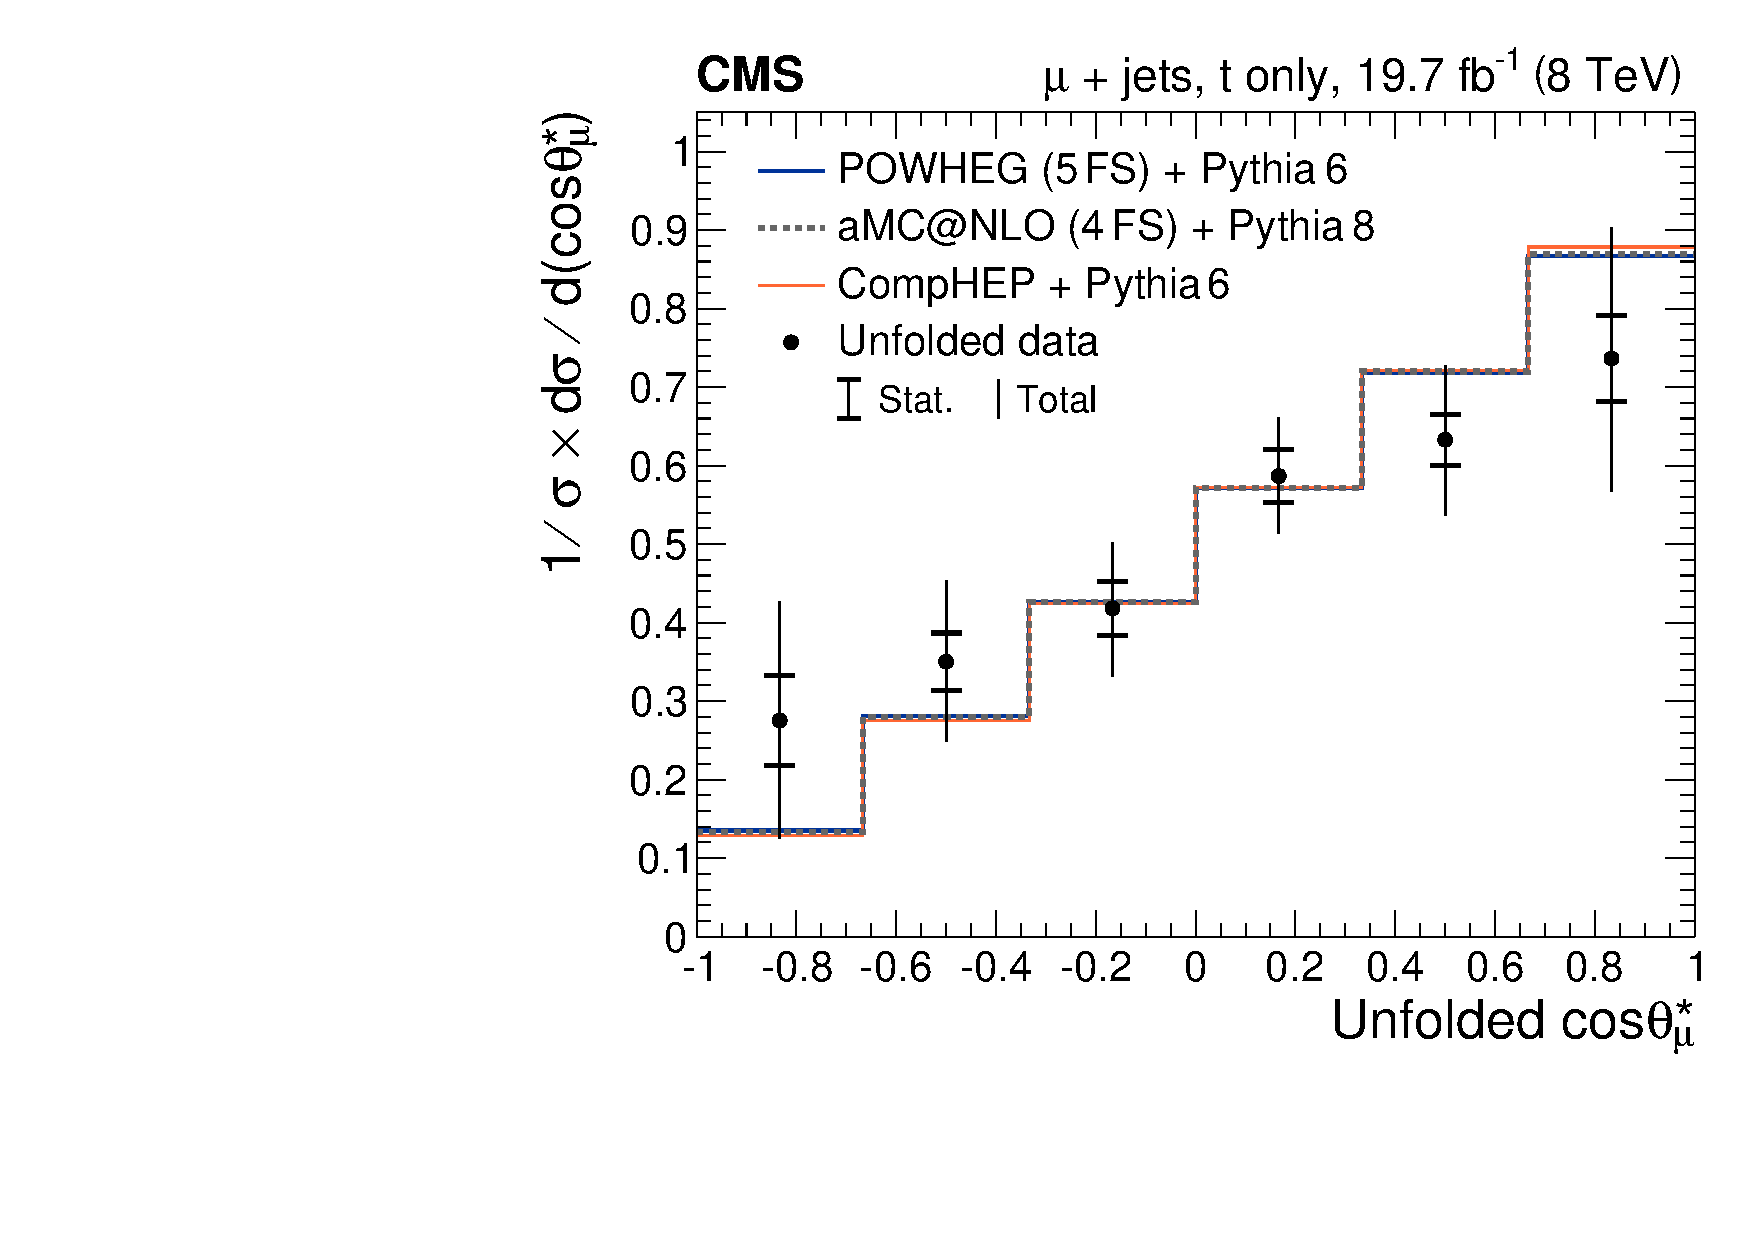
\includegraphics[width=0.48\textwidth]{figures/polarization/result/unfolded_mu_top.pdf}}
\hspace{0.02\textwidth}
\subfloat[]{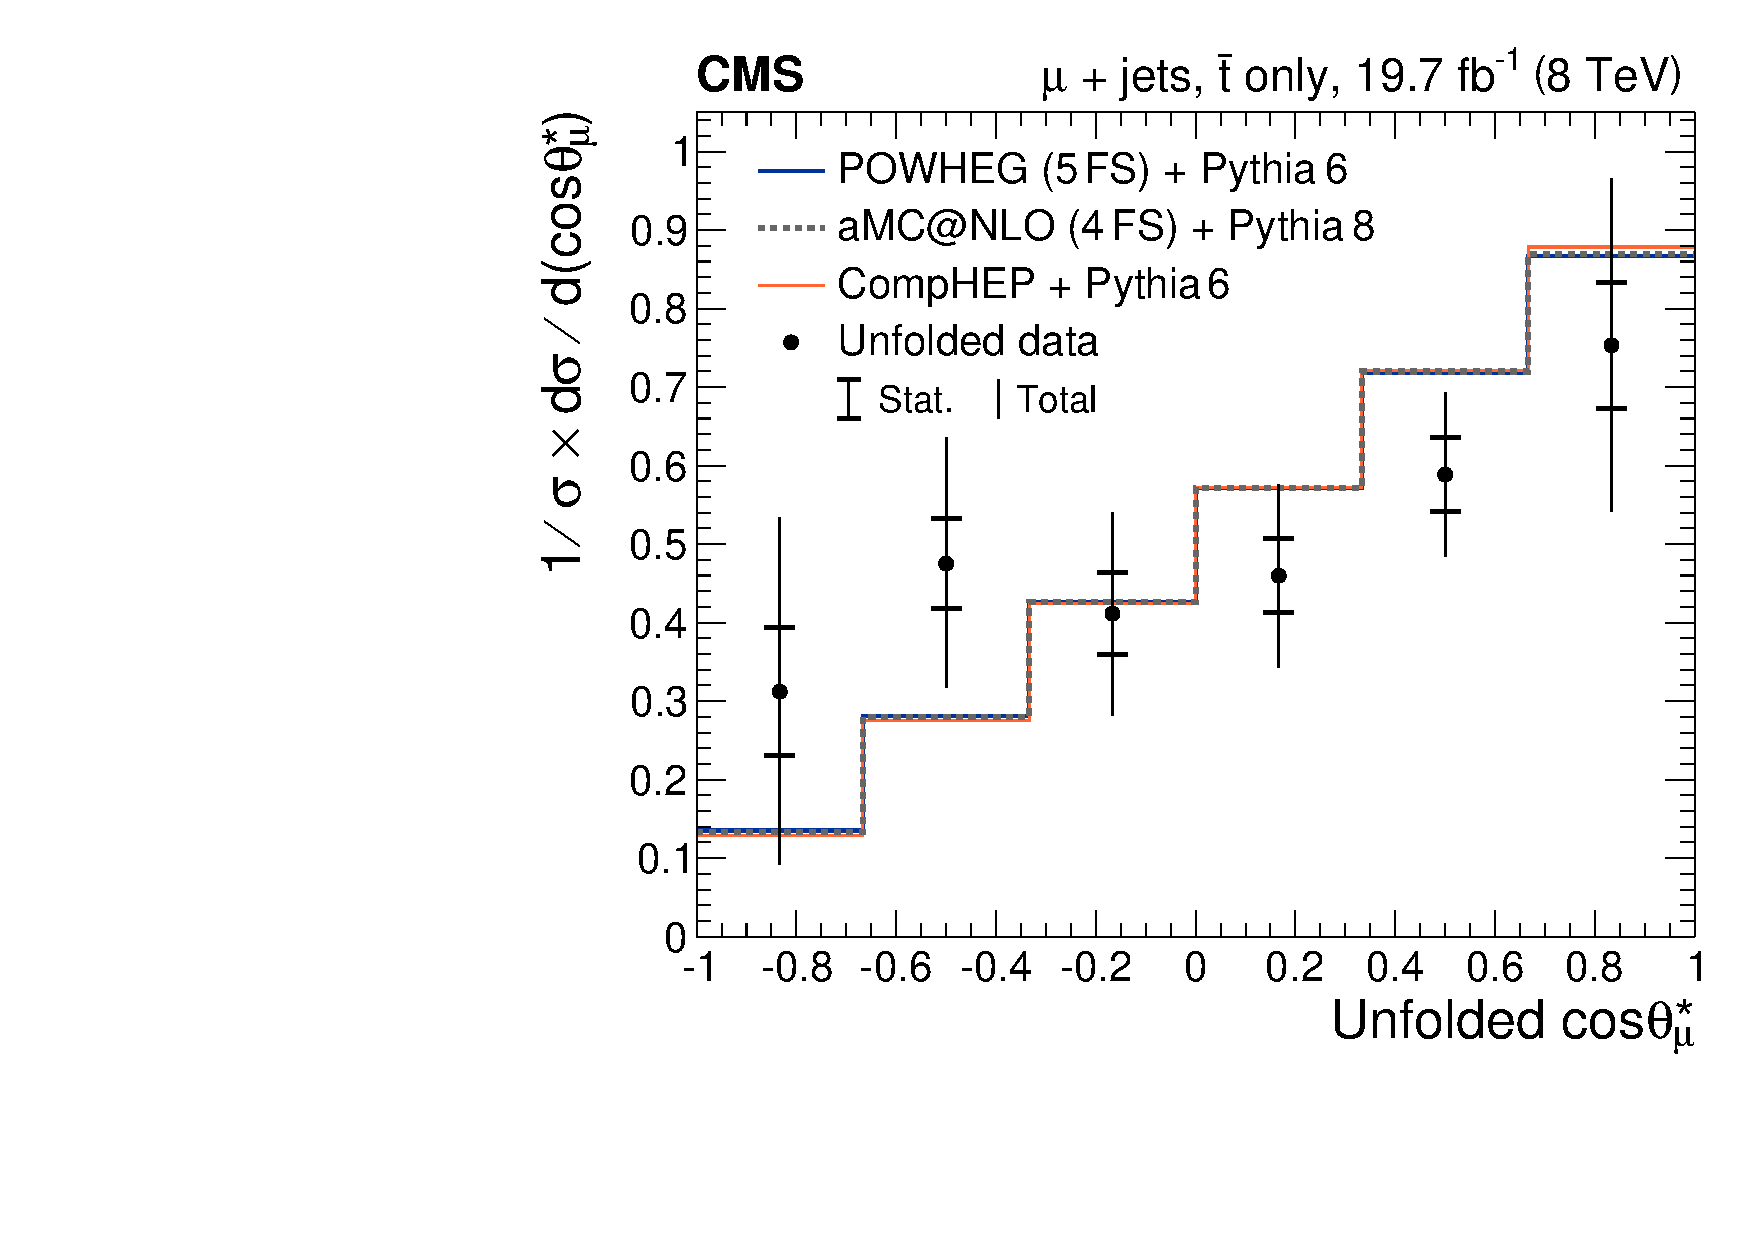
\includegraphics[width=0.48\textwidth]{figures/polarization/result/unfolded_mu_antitop.pdf}}\\
\subfloat[]{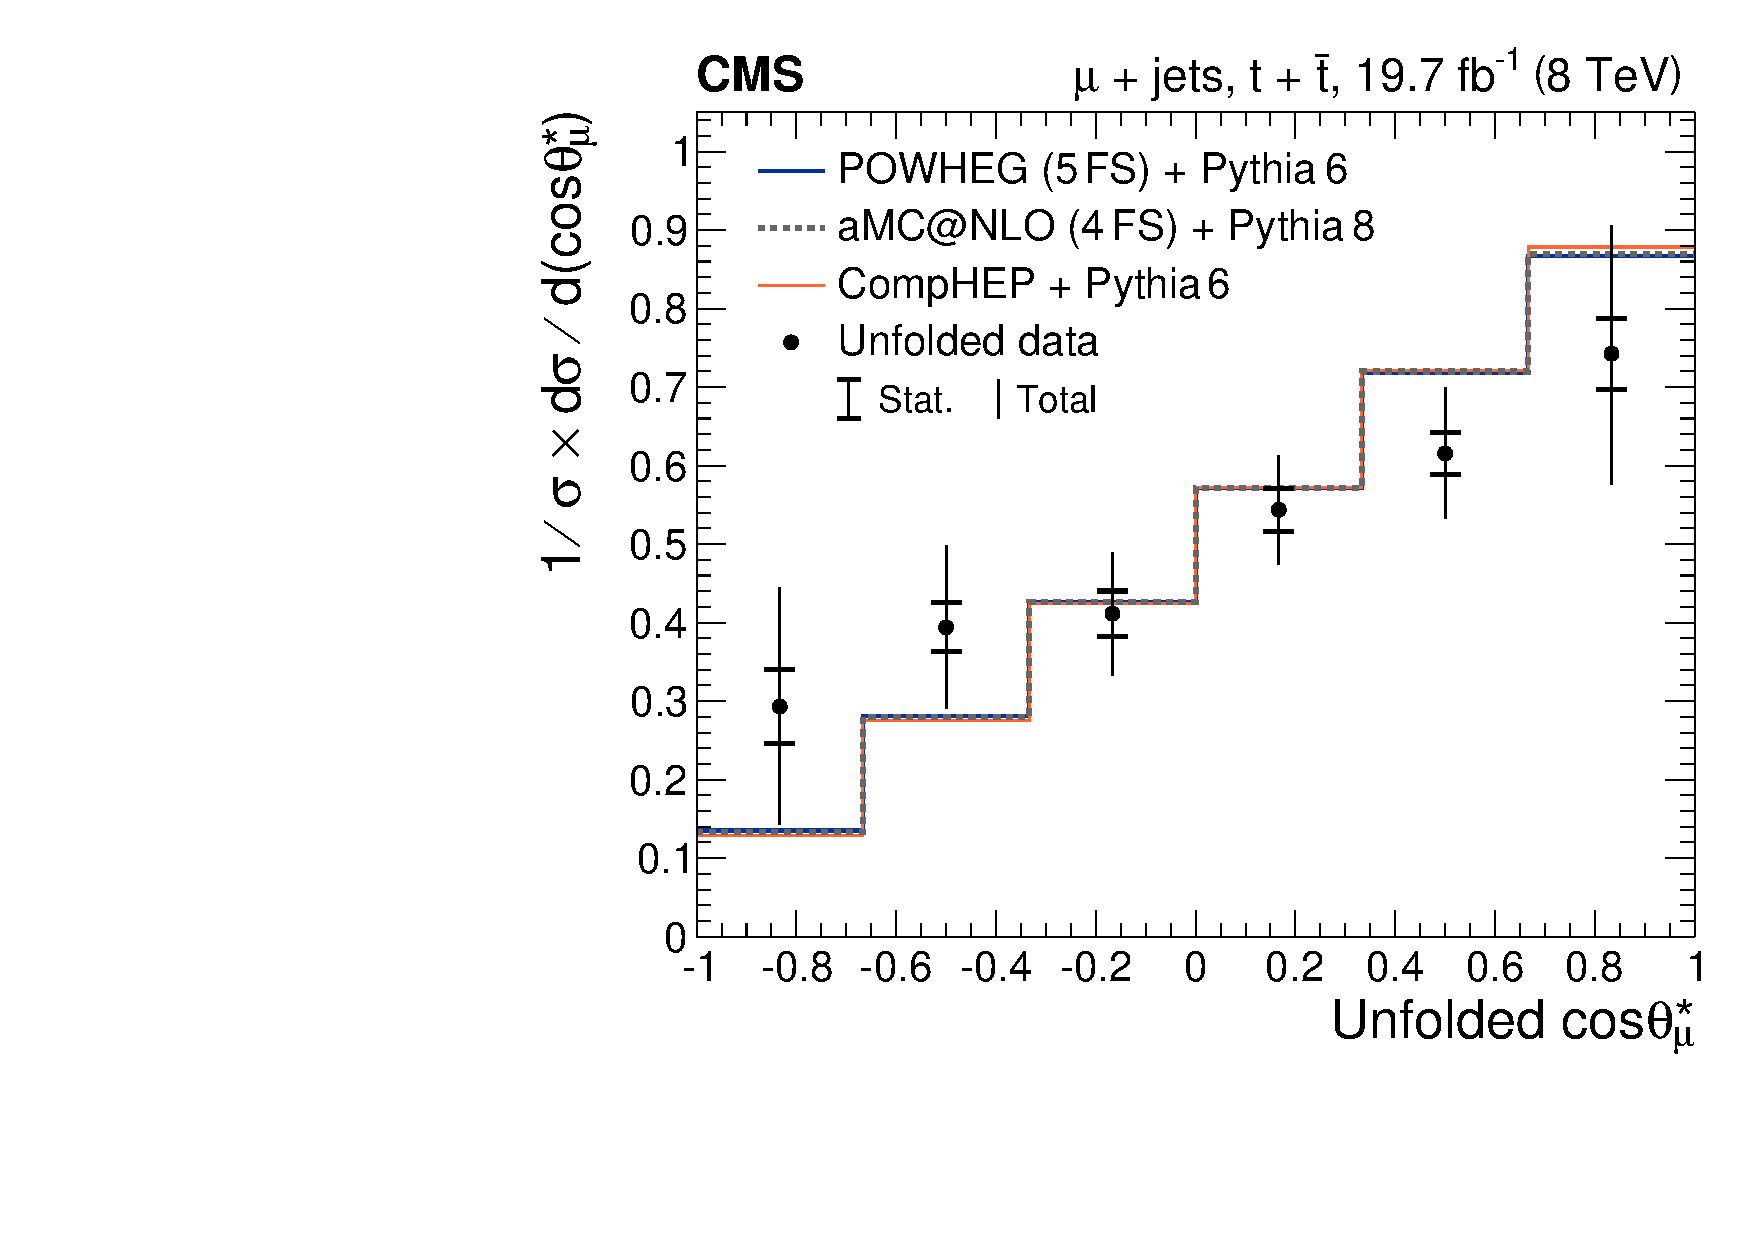
\includegraphics[width=0.48\textwidth]{figures/polarization/result/unfolded_mu.pdf}}
}


\newcommand{\AlResultCombined}{\ensuremath{\Big[26.0\pm 10.5 \Big]\cdot 10^{-2}}\xspace}
\newcommand{\AlResultCombinedStatSys}{\ensuremath{\Big[26.0\pm 2.6 \mathrm{(stat.)}\pm 10.2\mathrm{(syst.)} \Big] \cdot 10^{-2}} \xspace}
\newcommand{\AlResultCombinedPvalue}{\ensuremath{4.6\cdot 10^{-2}}\xspace}

\newcommand{\AlResultTop}{\ensuremath{\Big[29.0\pm 10.5 \Big]\cdot 10^{-2}}\xspace}
\newcommand{\AlResultTopStatSys}{\ensuremath{\Big[29.0 \pm 3.2 \mathrm{(stat.)} \pm 10.0\mathrm{(syst.)} \Big]\cdot 10^{-2}}\xspace}
\newcommand{\AlResultTopPvalue}{\ensuremath{7.9\cdot 10^{-2}}\xspace}

\newcommand{\AlResultAntiTop}{\ensuremath{\Big[21.1\pm 13.8 \Big]\cdot 10^{-2}}\xspace}
\newcommand{\AlResultAntiTopStatSys}{\ensuremath{\Big[21.1\pm 4.6\mathrm{(stat.)}\pm 12.6\mathrm{(syst.)} \Big]\cdot 10^{-2}}\xspace}
\newcommand{\AlResultAntiTopPvalue}{\ensuremath{5.0\cdot 10^{-2}}\xspace}


From data, we measure

\begin{align}
\AmuT          & = \AlResultTopStatSys = \AlResultTop , \\
\AmuTbar       & = \AlResultAntiTopStatSys = \AlResultAntiTop , \\
\AmuTplusTbar & = \AlResultCombinedStatSys = \AlResultCombined
\end{align}

using TUnfold. The measured asymmetries are compatible with a p-value of

\begin{align}
\AmuT:&\hspace{0.3cm} p(\mathrm{data |SM})          = \AlResultTopPvalue , \\
\AmuTbar:&\hspace{0.3cm} p(\mathrm{data |SM})      = \AlResultAntiTopPvalue , \\
\AmuTplusTbar:&\hspace{0.3cm} p(\mathrm{data |SM}) = \AlResultCombinedPvalue
\end{align}

with the SM value of $43.8\cdot 10^{-2}$ as predicted by \POWHEG.



\begin{align}
\AmuT          & = \Big[31.7\pm 3.7 \mathrm{(stat.)}\pm 10.9\mathrm{(syst.)} \Big]\cdot 10^{-2} = \Big[31.7\pm 11.2 \Big]\cdot 10^{-2} , \\
\AmuTbar       & = \Big[20.3\pm 5.7 \mathrm{(stat.)}\pm 15.0\mathrm{(syst.)} \Big]\cdot 10^{-2} = \Big[20.3\pm 16.0 \Big]\cdot 10^{-2} , \\
\AmuTplusTbar & = \Big[27.6\pm 3.1 \mathrm{(stat.)}\pm 11.1\mathrm{(syst.)} \Big]\cdot 10^{-2} = \Big[27.6\pm 11.5 \Big]\cdot 10^{-2} 
\end{align}

using the 2-bin analytic unfolding method as cross check.



%##############################################
\section{Limits on anomalous couplings}
%##############################################

topfit

combine: t-channel 8TeV~\cite{Khachatryan:2014iya}, Whelicity at 8TeV~\cite{Khachatryan:2016fky}


\myfigure{\label{fig:polarization-limits}Projections of limits on anomalous couplings and the top quark polarization for cases with free floating polarization~(violet) or when fixing the polarization to the anomalous couplings~(orange): (a)~left-handed vector couplings against polarization; (b)~right-handed vector coupling against polarization; (c)~left-handed tensor coupling against polarization; (d)~right-handed tensor coupling against polarization.}{
\subfloat[]{\adjincludegraphics[height=4.65cm,trim={0 0 {0.15\width} 0},clip]{figures/polarization/limits/Ptvl-nol.pdf}}
\subfloat[]{\adjincludegraphics[height=4.65cm,trim={0 0 {0.0\width} 0},clip]{figures/polarization/limits/Ptvr.pdf}}\\
\subfloat[]{\adjincludegraphics[height=4.65cm,trim={0 0 {0.15\width} 0},clip]{figures/polarization/limits/Ptgl-nol.pdf}}
\subfloat[]{\adjincludegraphics[height=4.65cm,trim={0 0 {0.0\width} 0},clip]{figures/polarization/limits/Ptgr.pdf}}
}
